\documentclass{beamer}

\usepackage[OT1]{fontenc}
\usepackage[utf8]{inputenc}
\usepackage[russian,english]{babel}
%%%% Additional part of preamble generated by package Sweave in RStudio
%% initial declaration for fonts
\usepackage[labelfont=bf]{caption}
\usepackage[font=small,labelfont=bf]{subcaption}


%% For tables
\usepackage{array}
\usepackage{longtable}
\usepackage{fullpage}
\usepackage{dcolumn}
\usepackage[flushleft]{threeparttable}
\usepackage{booktabs}
\usepackage[12hr]{datetime}
\usepackage[DIV=16]{typearea}
\usepackage{scrextend,booktabs}
\usepackage{tabulary}
\usepackage{multirow}
\usepackage[font=footnotesize]{caption}


%% Additional elements for figures and numbering added by Sweave
\usepackage{float}
\usepackage[sc]{mathpazo}
\usepackage{geometry}
\geometry{verbose,tmargin=2.5cm,bmargin=2.5cm,lmargin=2.5cm,rmargin=2.5cm}
\setcounter{secnumdepth}{2}
\setcounter{tocdepth}{2}
\usepackage{url}


%% Additional links for hyperref
\usepackage[unicode=true,pdfusetitle,
bookmarks=true,bookmarksnumbered=true,bookmarksopen=true,bookmarksopenlevel=2,
breaklinks=false,pdfborder={0 0 1},backref=false,colorlinks=false]
{hyperref}
\hypersetup{
	pdfstartview={XYZ null null 1}}

\usepackage{breakurl}
\usepackage{Sweave}


\title[dd?]
{Может ли обесценение}
\author{Suhas D. Parandekar}
\date[WB Workshop, 2020]{Returns to Education World Bank Workshop, 2020}

\begin{document}
	
%%%%%%%%%%	
\begin{frame}
	\titlepage
\end{frame}

%%%%%%%%%%	
\begin{frame}{Outline}
	\tableofcontents
\end{frame}
	
%%%%%%%%%%
\section{Motivation}

\subsection{Stylized fact about Human Capital in Russia}
\subsection{Time Trend in Returns to Education in Russia}

%%%%%%%%%%
\begin{frame}{Motivation}{Rates of Overall and Gender-wise Returns to Education in 1994-2018}
	\centering
	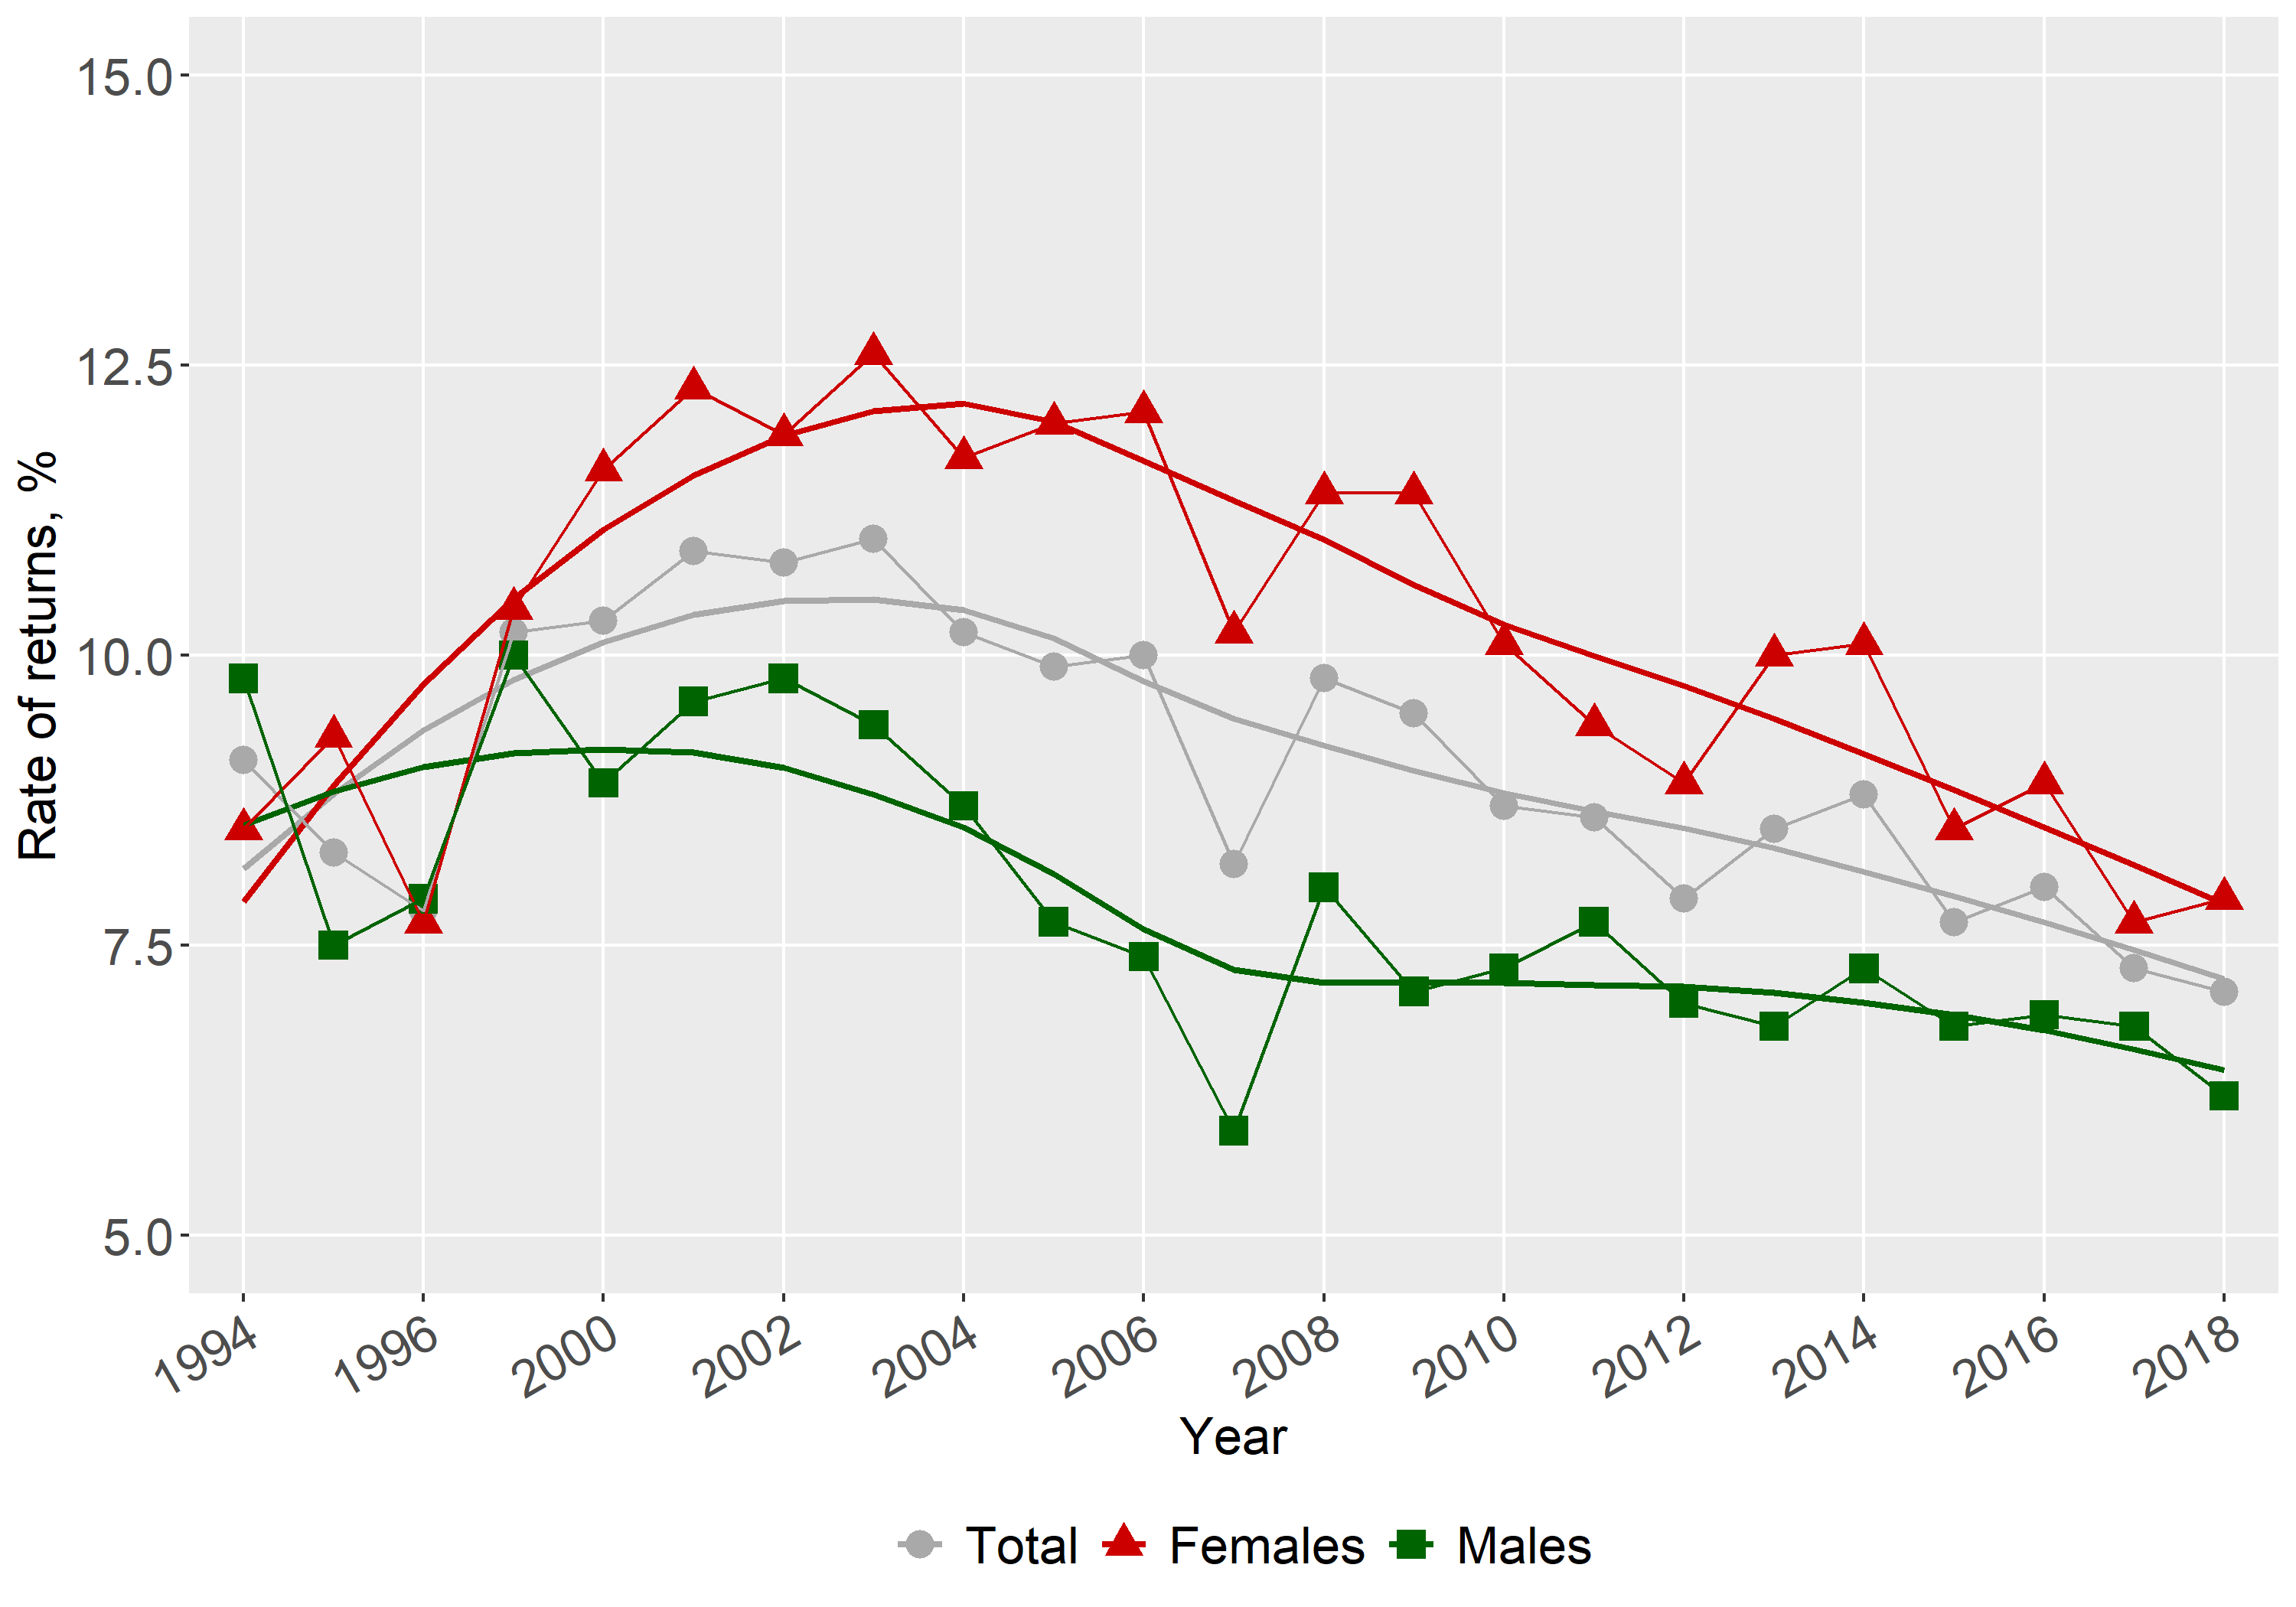
\includegraphics[width=260pt, height=200pt]{re_edu.png}
\end{frame}

%%%%%%%%%%
\begin{frame}{Results on Returns to Education in Russia}{Co-movement of Vocational Education and Higher Education by Gender}
	\begin{figure}
		\centering
		\subfloat[Females]{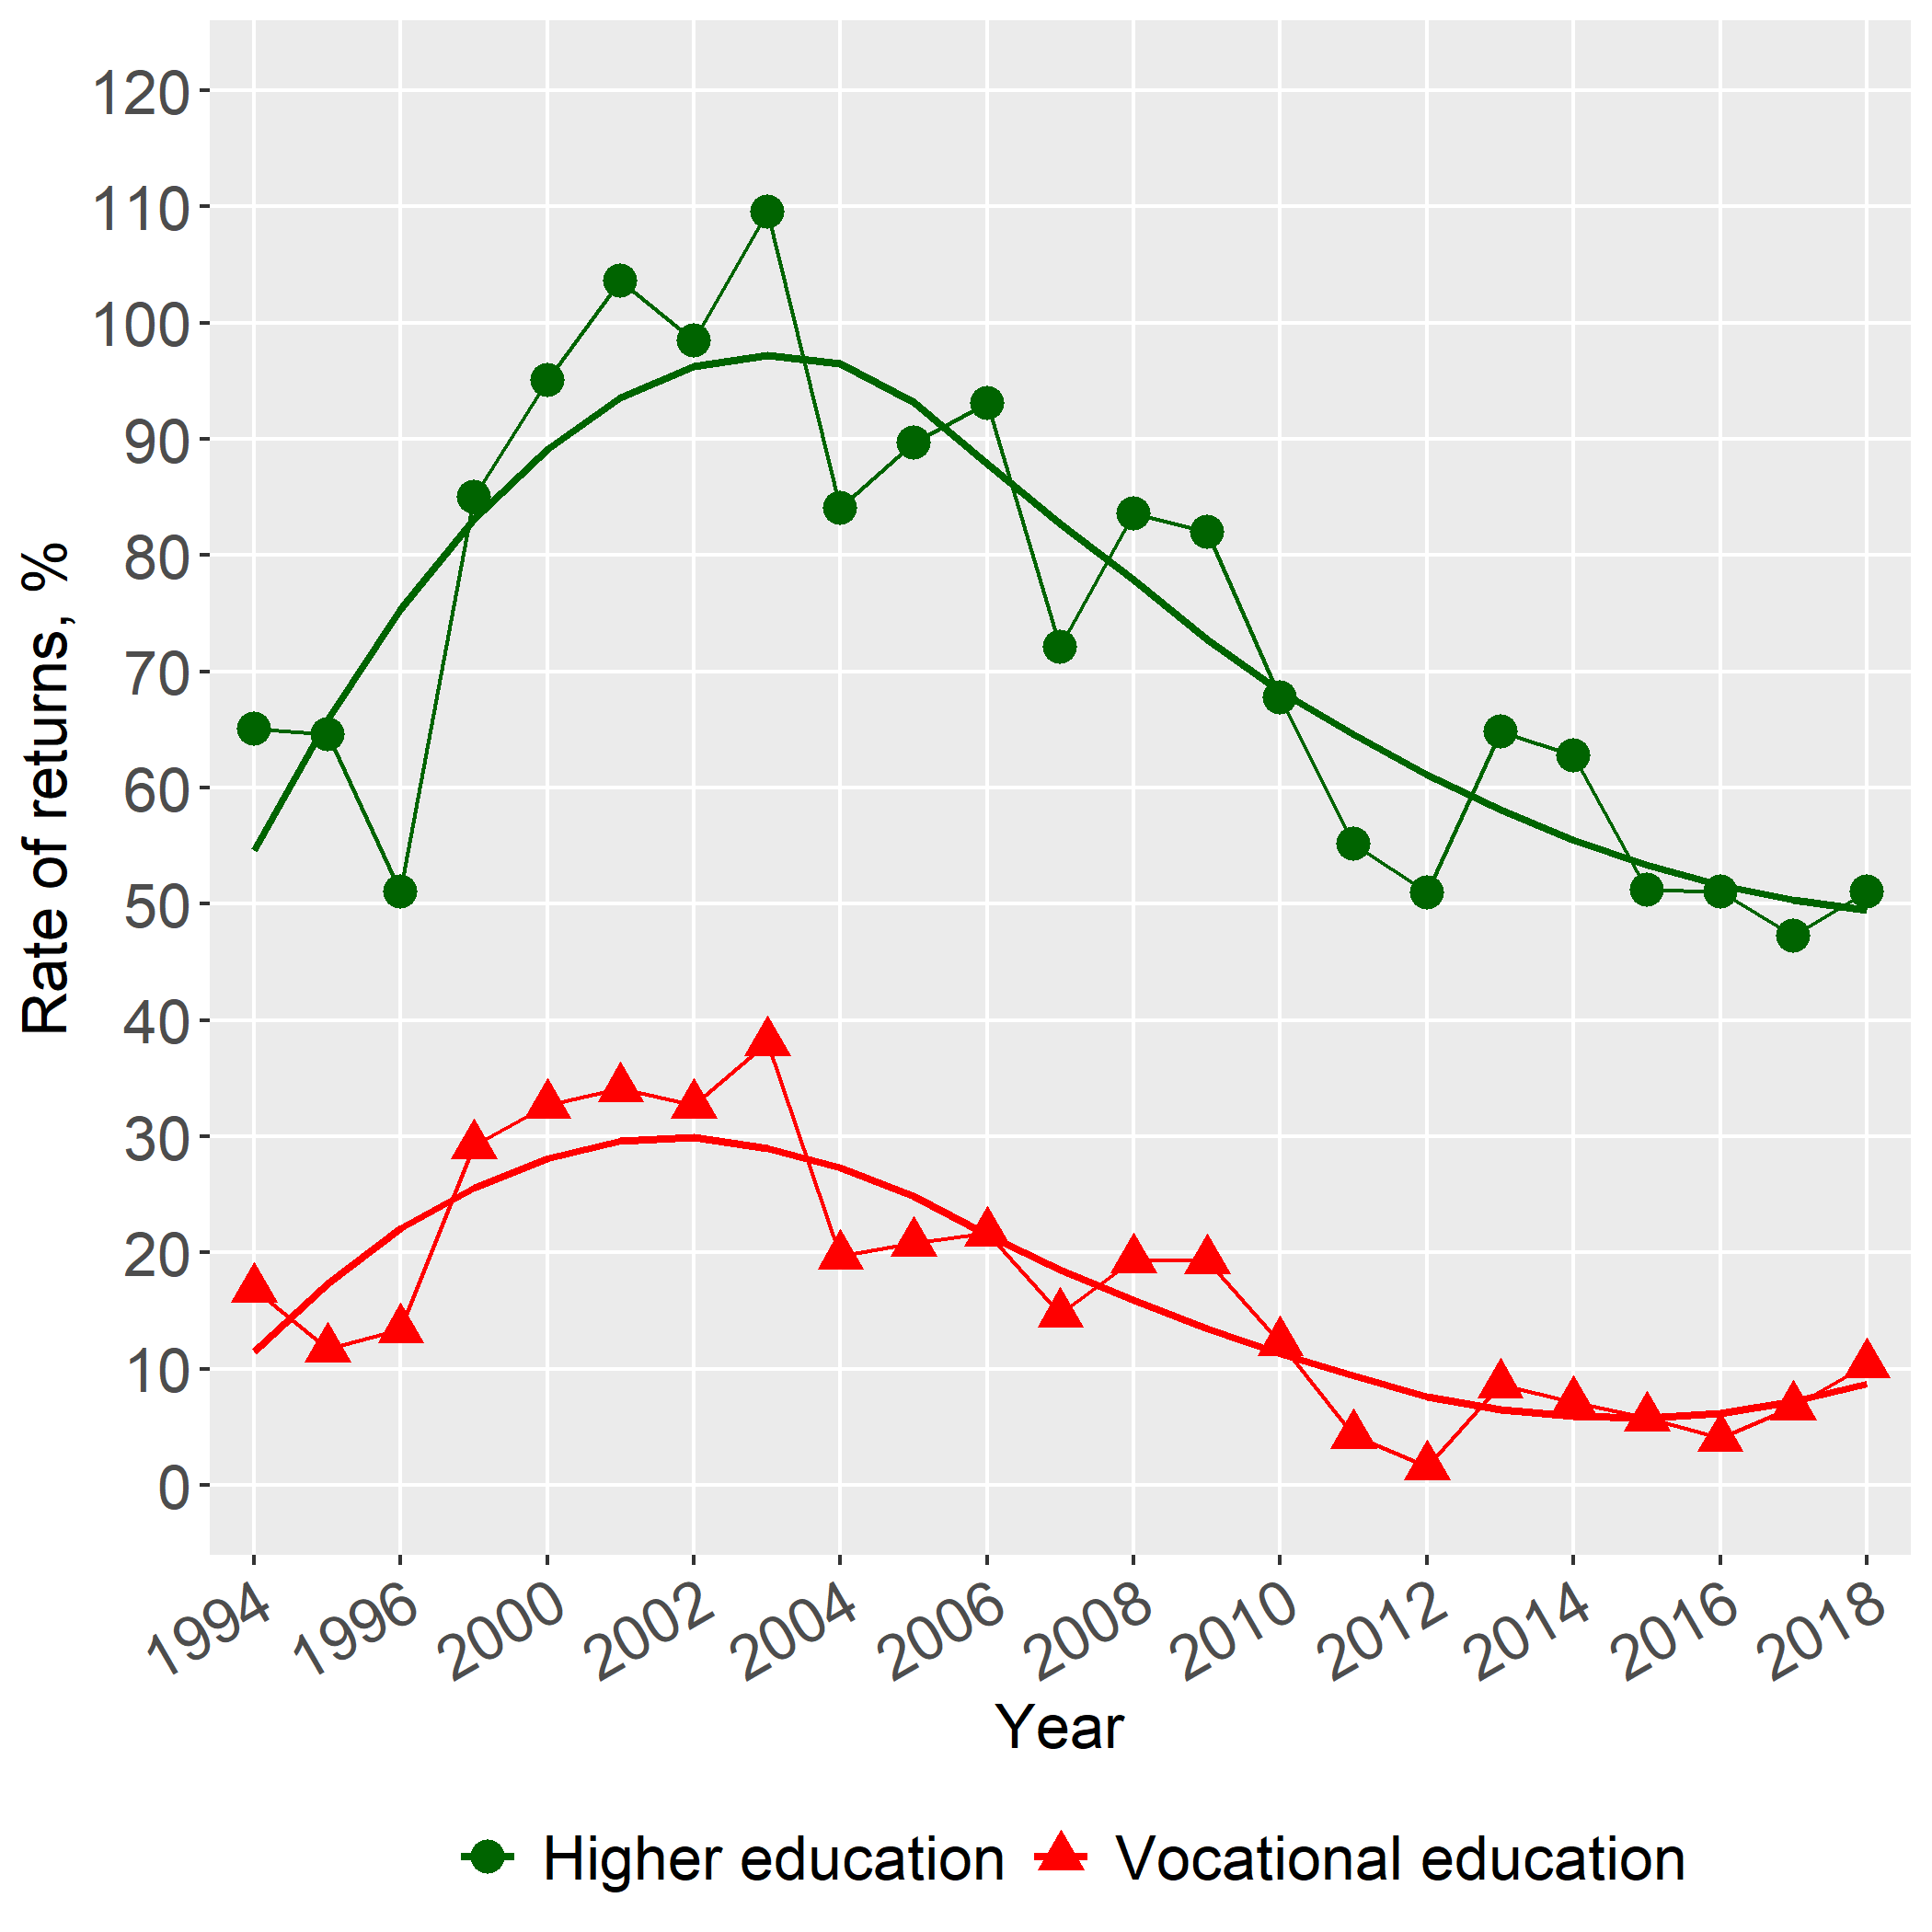
\includegraphics[width=150pt]{re_HE_f.png}}
		\hfill
		\subfloat[Males]{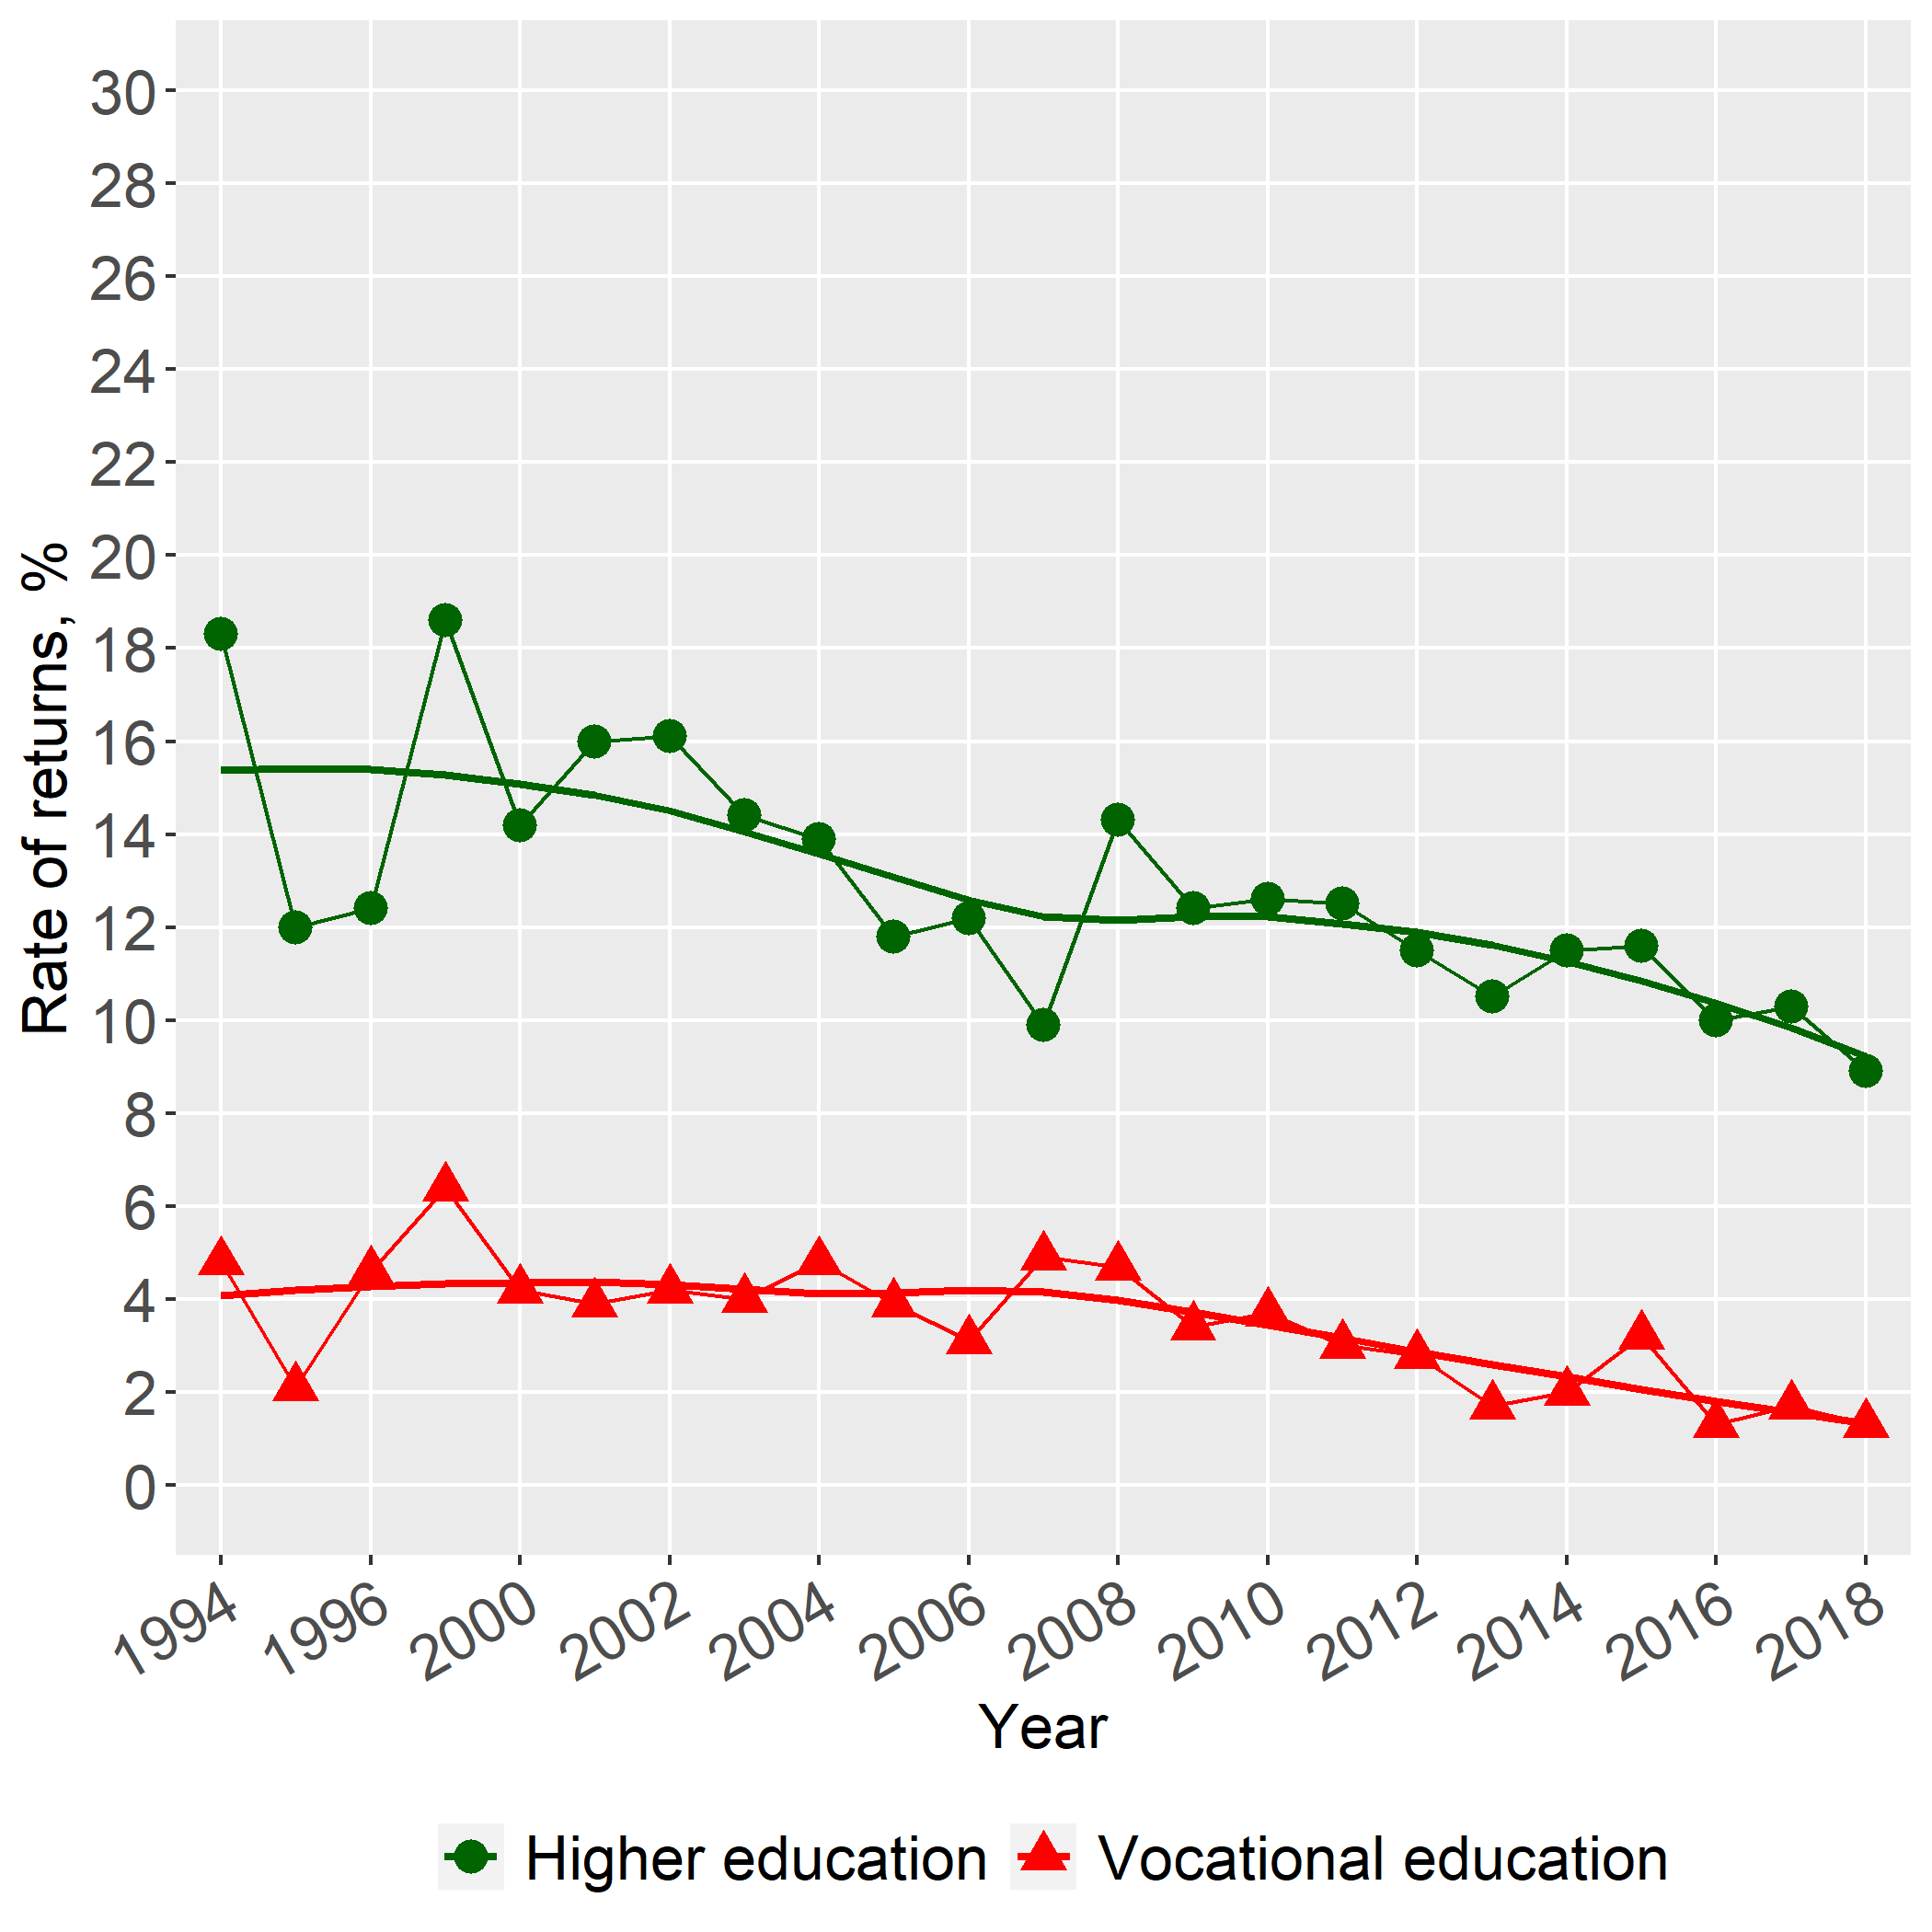
\includegraphics[width=150pt]{re_HE_m.png}}
	\end{figure}
	\begin{itemize}
		\vspace*{-0.2in}
		\item Returns for males are almost flat.
		\item Returns for females show a \textit{concave} pattern.
	\end{itemize}
\end{frame}



%%%%%%%%%%
\begin{frame}{Motivation}{Peak in Enrollment in University Education (HSE Yearbook)}
\begin{figure}
	\centering
	\vspace*{-0.2in}
	\hspace*{-0.3in}
	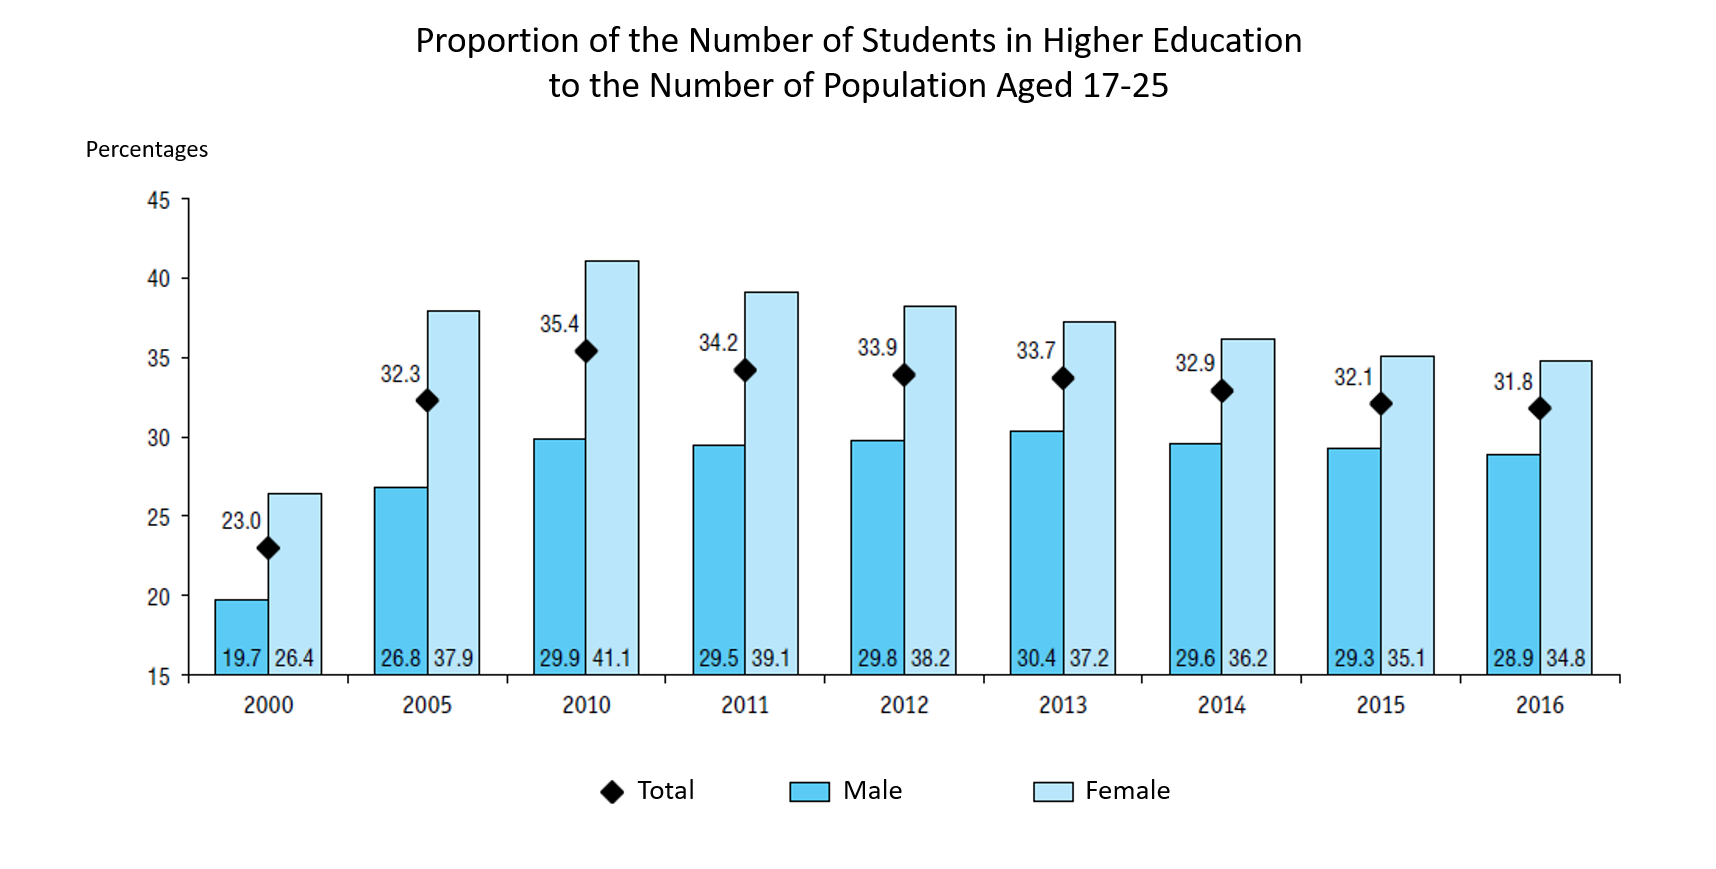
\includegraphics[width=350pt]{graph_1b.png}
\end{figure}
\end{frame}
	

%%%%%%%%%%
\section{Depreciation of Human Capital in Russia}
\subsection{Analytical Treatment of Depreciation}

%%%%%%%%%%
\begin{frame}{Depreciation of Human Capital in Russia}{Neuman-Weiss Vintage Effects by Education Levels}
\begin{figure}
	\centering
	\subfloat[Higher Education]{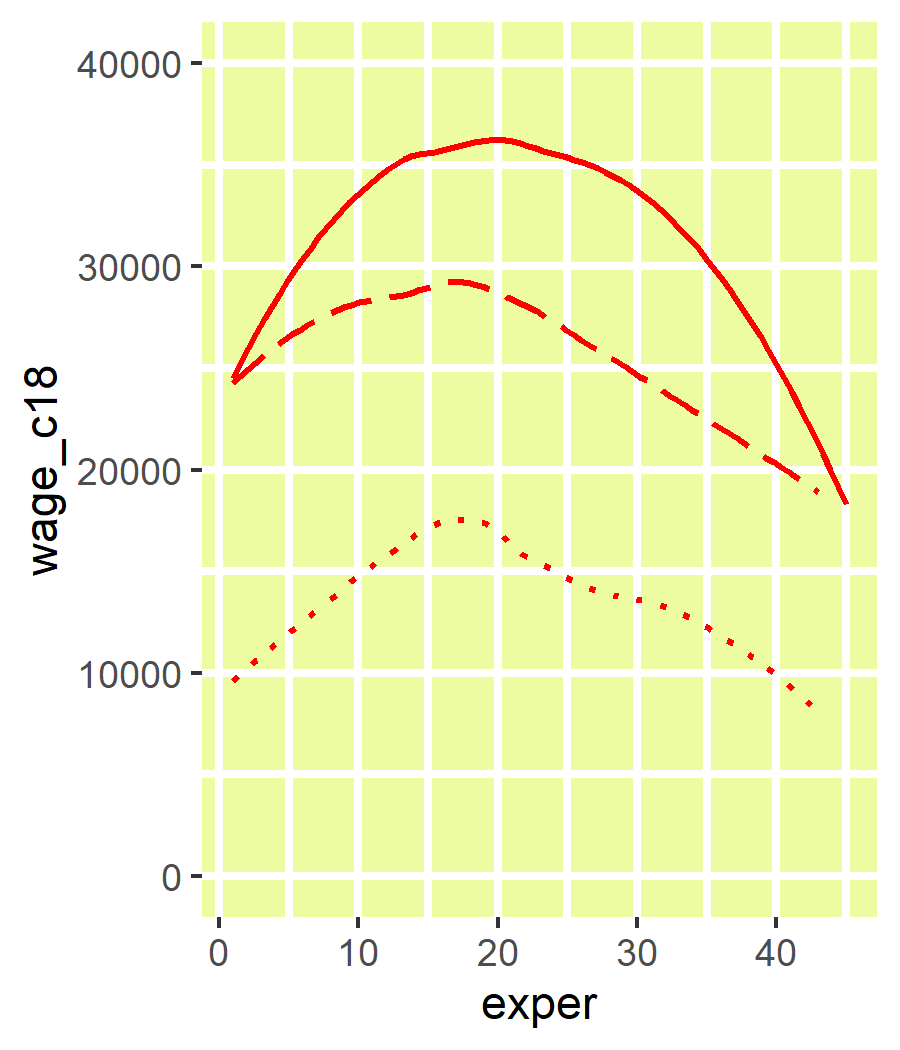
\includegraphics[width=110pt]{dp01_he.png}}
	\hfill
	\subfloat[Vocational Education]{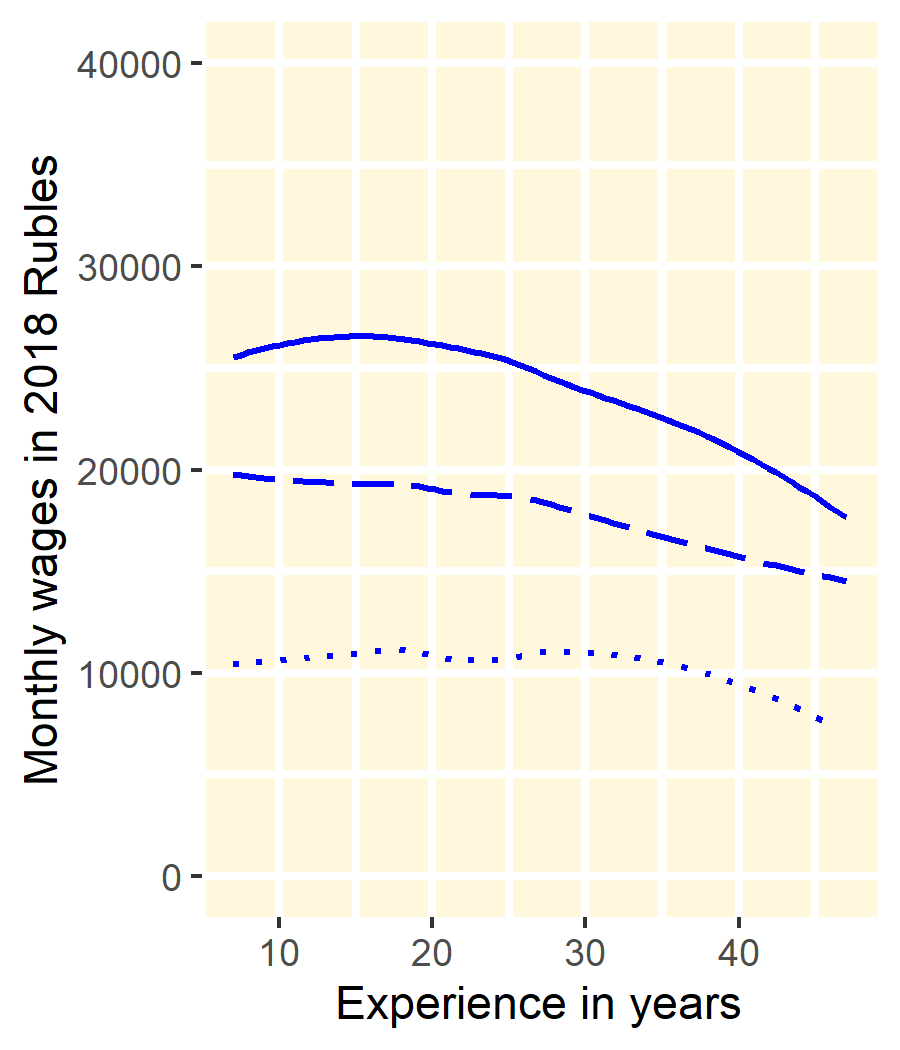
\includegraphics[width=110pt]{dp01_ve.png}}
	\hfill
	\subfloat[Secondary Education]{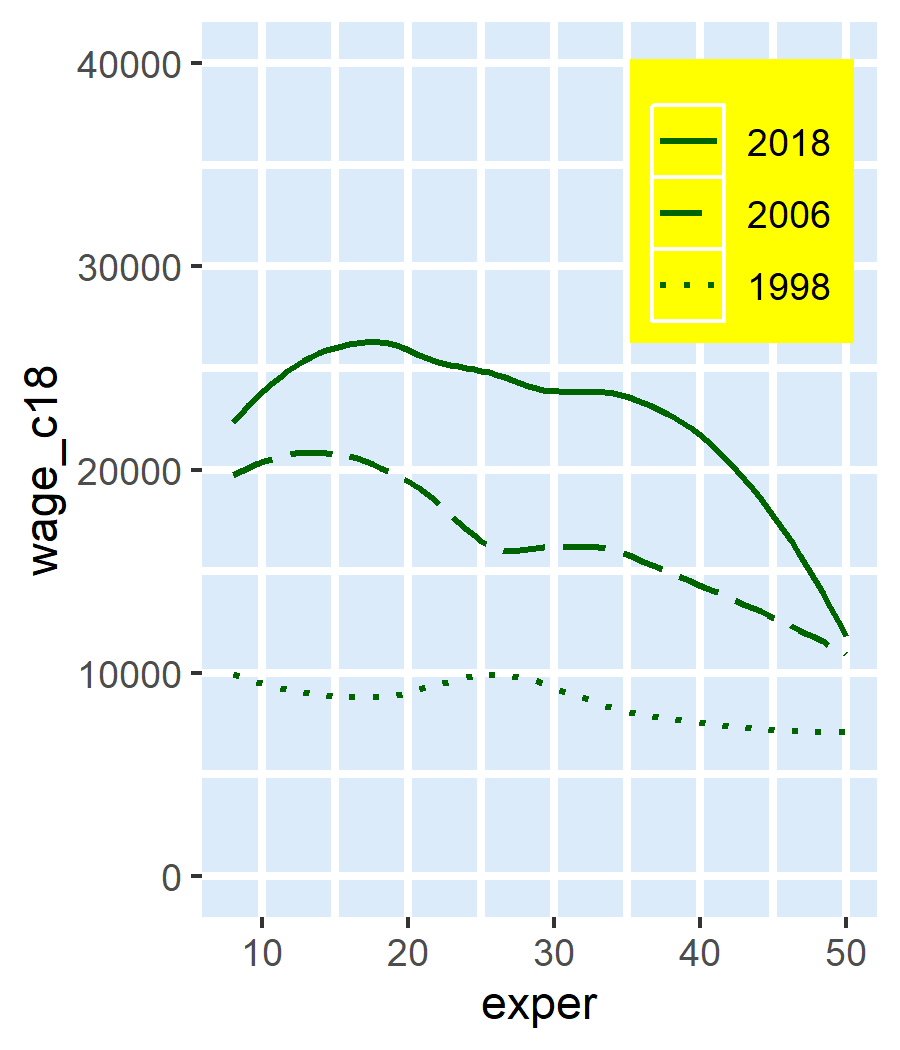
\includegraphics[width=110pt]{dp01_se.png}}
\end{figure}
\begin{itemize}
	\item A clear concave downwards profile is only for Higher Education.
	\item The concave tendency is less pronounced for the other two levels of Vocational and Secondary education.
	\item However, we need a more rigorous treatment of this issue.
\end{itemize}
\end{frame}

\begin{frame}{Depreciation of Human Capital in Russia}{Analytical Treatment of Depreciation}
	Two kinds of depreciation or \textit{loss of productive potential of human capital} \citep{neuman_091._1995}:
	\begin{itemize}
		\item \textbf{External depreciation} (``obsolescence" or ``vintage effect"): due to an overall upgrading of technology or the operation of other market forces that lowers the value of education or training obtained in a previous period.
		\item \textbf{Internal depreciation:} due to deterioration of physical and mental abilities of an individual due to the progression of a person's age.
	\end{itemize}
\end{frame}

%%%%%%%%%%
\begin{frame}{Depreciation of Human Capital in Russia}{Murillo Methods}
\begin{itemize}
	\item \citet{murillo_172._2006} implemented a variation of the \citet{neuman_091._1995} model with a focus on
	empirical implementation to Spain.
	\item In a nutshell, the model can be expressed as follows:
	
	\begin{equation}
	log(W) = \alpha +  \beta_{1}S + \pi_{1}TS + \beta_{2}T + \pi_{2}T^{2} 
	\end{equation}
	where $T$ is years of experience, $S$ is years of schooling, $\alpha$, $\beta_{1}$, $\beta_{1}$, $\pi_{1}$, $\pi_{2}$ are regression coefficients.
	\vspace{2pt}
	\item The depreciation rate during $T$ years applied to schooling can be computed as $\pi_{1}S $ and the depreciation rate applied to experience as $ 2\pi_{2}T$.
\end{itemize}
\end{frame}

%%%%%%%%%%
\subsection{Estimation Results}
\begin{frame}{Depreciation of Human Capital in Russia}{Initial Results for the Depreciation Rate (DR) by Years}
	\fontsize{7}{18}\selectfont
	\begin{tabularx}{\textwidth}{rlrrrrrrc}
		\hline
		& \textbf{Statistic} & \textbf{1994} & \textbf{1998} & \textbf{2003} & \textbf{2006} & \textbf{2012} & \textbf{2018} &  \\ 
		\hline
		1 & Experience, mean   & 21.41 & 22.32 & 22.20 & 22.24 & 22.52 & 22.52 & \\
		2 & Education, mean & 12.70 & 12.69 & 12.79 & 12.79 & 12.95 & 13.27 &\\
		\hline
		3 & DR Experience, \% & 1.87 & 1.55 & 1.04 & 0.50 & 1.37 & 1.63 & 
		\graph{1}{1}{C:/Country/Russia/Data/SEASHELL/SEABYTE/Edreru/wp1/sparklines/all2-1} \\ 
		4 & DR Education, \% & 2.80 & 2.71 & 0.11 & 0.00 & 0.00 & 0.00 &
		\graph{1}{1}{C:/Country/Russia/Data/SEASHELL/SEABYTE/Edreru/wp1/sparklines/all2-2} \\ 
		5 & DR Human Capital, \% & 4.67 & 4.26 & 1.15 & 0.50 & 1.37 & 1.63 & 
		\graph{1}{1}{C:/Country/Russia/Data/SEASHELL/SEABYTE/Edreru/wp1/sparklines/all2-3}\\ 
		\hline
	\end{tabularx}

\end{frame}

%%%%%%%%%%
\subsection{Arrazola's Non-Linear Least Squares Approach}
	\subsection{Estimation Results}
%%%%%%%%%%
\begin{frame}{Depreciation of Human Capital in Russia}{Non-Linear Least Squares Estimates: Whole Sample}
	\fontsize{8}{10}\selectfont
	\begin{itemize}
		\item	\citet{arrazola_132b._2005} developed an alternative \textit{Non-Linear Least Squares} approach on the issue of human capital depreciation.
	\end{itemize}
		\fontsize{5}{11}\selectfont
		\keepXColumns
		\begin{tabularx}{\textwidth}{clccccccc}
			\hline
			& \textbf{Parameter} & \textbf{1994} & \textbf{1998} & \textbf{2003} & \textbf{2006} & \textbf{2012} & \textbf{2018} & \\ 
			\hline
			& \textbf{\begin{tabular}[l]{@{}l@{}} Human Capital \\ Depreciation: Whole Sample \end{tabular}} & 0.0246 & 0.0208 & 0.0093 & -0.0040 & 0.0369 & 0.0459 & 
			\graph{1}{1}{C:/Country/Russia/Data/SEASHELL/SEABYTE/Edreru/wp1/sparklines/Weber_sprk_all2-1}\\ 
			
			&  & (0.0052) & (0.0043) & (0.0050) & (0.0058) & (0.0043) & (0.0051) & \\ 
			\hline
			
			& \textbf{\begin{tabular}[l]{@{}l@{}} Human Capital \\ Depreciation: Female Sample \end{tabular}} & 0.0275 & 0.0260 & 0.0156 & 0.0065 & 0.0197 & 0.0249 & 
			\graph{1}{1}{C:/Country/Russia/Data/SEASHELL/SEABYTE/Edreru/wp1/sparklines/Weber_sprk_f2-1}\\ 
			&  & (0.0060) & (0.0042) & (0.0038) & (0.0044) & (0.0036) & (0.0036) & \\ 
			\hline
			
			& \textbf{\begin{tabular}[l]{@{}l@{}} Human Capital \\ Depreciation: Male Sample \end{tabular}} & 0.0261 & 0.0168 & -0.0020 & 0.0015 & 0.0595 & 0.0511 & 
			\graph{1}{1}{C:/Country/Russia/Data/SEASHELL/SEABYTE/Edreru/wp1/sparklines/Weber_sprk_m2-1}\\ 
			&  & (0.0067) & (0.0059) & (0.0082) & (0.0095) & (0.0063) & (0.0069) & \\
			\hline
			
		\end{tabularx}
	\fontsize{8}{10}\selectfont
\begin{itemize}
	\item The sparklines indicate a similar roughly\textbf{ U-shaped pattern} for depreciation as reported for Murillo's estimations, with depreciation of human capital first declining and then increasing again. 
	\item This supports the narrative that the observed increase and then decrease in returns to education in the Russia may be explained through the	effect of depreciation.
\end{itemize}
\end{frame}		

%%%%%%%%%%
\section{Further Exploration of Depreciation}
	\subsection{Depreciation and the Gender Dimension}

%%%%%%%%%%
\begin{frame}{Further Exploration of Depreciation}{Depreciation and the Gender Dimension}
	\begin{itemize}
		\item The Neuman and Weiss model provides an estimation of the depreciation rate for human	capital, but by itself is unable to identify how much of that depreciation is \textit{external} or \textit{internal}.
		\item Examining differences in depreciation rate by the \textbf{segregation classification} helps solve this problem based on a conjecture.
		\item The conjecture is that \textit{external depreciation} would have a greater affect by \textbf{industry sector}, as technological change would propagate more rapidly through a sector rather than through \textbf{occupations}, which are dispersed across sectors.
		\item Occupation is related to education and changes in education propagate slower. Industries include heterogeneous education groups, while occupations are more homogeneous, and hence market changes affect industries quicker.
	\end{itemize}
\end{frame}	
	
%%%%%%%%%%
\begin{frame}{Further Exploration of Depreciation}{Average Human Capital Depreciation Rates (DR) by Female- and Male-dominated Industries and Occupations, RLMS 2018}
		\fontsize{9}{11}\selectfont
		\centering 
		\label{tab:3.3} 
		\begin{tabularx}{\textwidth}{cl|cc|cc}
			\hline
			& \textbf{Statistic}
			& \textbf{\begin{tabular}[c]{@{}c@{}} Female-\\dominated \\ industries \end{tabular}}
			& \textbf{\begin{tabular}[c]{@{}c@{}} Male-\\dominated \\ industries \end{tabular}}
			& \textbf{\begin{tabular}[c]{@{}c@{}} Female-\\dominated \\ occupations \end{tabular}}
			& \textbf{\begin{tabular}[c]{@{}c@{}} Male-\\dominated \\ occupations \end{tabular}} \\ 
			\hline
			1 & Experience, mean  & 23.45 & 22.97 & 21.67 & 23.48 \\ 
			2 & Education, mean & 14.06 & 13.01 & 13.67 & 12.67 \\ 
			\hline
			3 & DR Experience, \% & 0.89 & 1.82 & 1.55 & 1.40 \\ 
			4 & DR Education, \% & 0.00 & 0.00 & 0.00 & 0.00 \\ 
			5 & DR Human Capital, \% & \textcolor{red}{0.89} & \textcolor{red}{1.82}
			 & \textcolor{blue}{1.55} & \textcolor{blue}{1.40} \\ 
			\hline
		\end{tabularx}
	 \fontsize{8}{10}\selectfont
	\begin{itemize}
		\item DR is higher for male-dominated \textbf{industries} \textit{(e.g., engineering and technology-oriented sectors)} compared to the female-dominated ones \textit{(e.g., administration, services, and education)}.
		\item But DR does not appear to vary across male-dominated \textit{(e.g., science and engineering professionals, stationary plant, and machine operators)} and female-dominated \textit{(e.g., personal care workers, teaching professionals, sales workers)} \textbf{occupational groupings}.
		\item This means that internal depreciation is the same for all individuals, but external depreciation is greater in male-dominated industries. 
	\end{itemize}
\end{frame}

%%%%%%%%%%	
\subsection{Depreciation and Occupational Routineness}

%%%%%%%%%%
\begin{frame}{Further Exploration of Depreciation}{Depreciation and Occupational Routineness}
	\begin{itemize}
		\item In light of a discussion about computers and robots taking over routine-oriented jobs, we compare DR between \textbf{jobs and sectors} using 2 measures \citep{mihaylov_152._2019}:
			\begin{itemize}
				\item \textbf{Net Routine Task Intensity}, showing vulnerability to automation of tasks performed as part of a job.   
				\item \textbf{Gross Non-Routiness Measure}, reflecting the opposite characteristic.
			\end{itemize}
		\item These measures are based on the textual analysis of jobs description in the ISCO-08 classification.
	\end{itemize}
\end{frame}

%%%%%%%%%%
\begin{frame}{Further Exploration of Depreciation}{Average Human Capital Depreciation Rates (DR) by Routineness Classification, RLMS 2018}
\fontsize{8}{10}\selectfont
\begin{table}[H]
	\centering
	\begin{tabular}{cl|ccc|cccccc}
		\hline
		& \textbf{Statistic} & \textbf{High} & \textbf{Low} & \textbf{Medium} & \textbf{High} & \textbf{Low} & \textbf{Medium} \\ 
		\hline
		& & \multicolumn{3}{c|}{\textbf{Net Routine Task Intensity}} & \multicolumn{3}{c} {\textbf{Gross Non-Routiness Measure}} \\
		\hline
		2 & Experience, mean  & 21.44 & 22.79 & 22.76 & 22.94 & 22.22 & 22.05 \\ 
		3 & Education, mean & 12.86 & 13.67 & 12.8 & 13.66 & 12.76 & 13.02 \\ 
		\hline
		4 & DR Experience, \% & 1.8 & 1.5 & 1.64 & 1.62 & 1.73 & 1.48 \\ 
		5 & DR Education, \% & 0 & 0 & 0 & 0 & 0 & 0 \\ 
		6 & DR Human Capital, \% & \textcolor{blue}{1.8} & \textcolor{blue}{1.5} & \textcolor{blue}{1.64} & \textcolor{blue}{1.62} & \textcolor{blue}{1.73} & \textcolor{blue}{1.48} \\ 
		\hline
	\end{tabular}
\end{table}
\fontsize{12}{12}\selectfont
	\begin{itemize}
	\item DR explained by experience does not differ substantially between people with jobs with varying routine task intensity. 
	\item The same outcome also applies to workers varying in the degree of non-routine content at their jobs.
	\item This means both external and internal depreciation types are the same across occupational groups generated on the basis of routineness intensity.
\end{itemize}
\end{frame}

%%%%%%%%%%

%%%%%%%%%%
\section*{Key Policy Issues}
\begin{frame}{Key Policy Issues}
	\fontsize{12}{17}\selectfont
	\begin{itemize}
	\item Benefits to society from human capital investment also depends on what happens to human capital after the schooling period. 
	\vspace{1cm}
	
	\item Human capital depreciation in the Russian Federation may have strong effect on returns to education, which in turn drive people's decisions for further education. 
	\end{itemize}
\end{frame}

\begin{frame}{Key Policy Issues}
	\fontsize{12}{17}\selectfont
	\begin{itemize}
		\item Policy to reduce \textbf{internal depreciation} includes incentives to individuals and firms to invest in on-the-job training and reskilling. 
		\vspace{1cm}
		
		\item Policy to reduce \textbf{external depreciation} would focus on curriculum/content of education: creativity and problem-solving skills; learning how to learn.
	\end{itemize}
\end{frame}


\end{document}
